\documentclass{article}
\usepackage{amsfonts}
\usepackage{amsmath}
\usepackage{listings}
\usepackage{graphicx}
\usepackage{subfig}
\author{Gwylim Ashley}
\title{A comparison of the Metropolis and Wang-Landau algorithms applied to the Potts model}
\begin{document}
\maketitle
\begin{abstract}
We discuss the advantages and limitations of the Metropolis and Wang-Landau algorithms as applied to physical systems.
In particular, we use the example of the Potts model, which exhibits a phase transition.
We find that the shape of the Boltzmann distribution near the phase transition leads to slow convergence using the Metropolis algorithm for large lattices.
Some general discussion of these algorithms is also included.
\end{abstract}
\tableofcontents
\section{Introduction}
Any general method to determine information about a thermodynamic system must look at the microstates of the system.
For example, to calculate $\langle E\rangle$ at some temperature, we need to calculate $\sum_s E(s)e^{-\beta E(s)}$.
However, for any system of reasonable size this will be infeasible, since the number of microstates is very large.

Hence instead of looking at all the microstates we can instead look at a representative sample.
For example, to calculate $\langle E\rangle$, we could choose at random a subset $S$ of states, and calculate $\sum_{s\in S}E(s)e^{-\beta E(s)}$.
However, in general this will not give good results: the majority of the microstates will not contribute much to this sum, so we will still need a very large sample.\footnote{In particular, selecting microstates uniformly at random is typically equivalent to selecting from a Boltzmann distribution with $T = \infty$. For most systems this will not give good results.}

A better approach is to use a \emph{random walk}.
Here we consider the microstates as a graph, with edges between microstates that are ``close'' in some sense.
We perform a random walk on this graph, and by weighting our random walk appropriately, we can obtain a more useful sample of microstates.

In this project two algorithms making use of this general approach are discussed: the Metropolis algorithm and the Wang-Landau algorithm.
The Metropolis algorithm (also known as the Metropolis-Hastings algorithm) is a general technique for sampling from certain types of probability distributions; here we will apply it to a physical system and obtain the Boltzmann distribution.
The Wang-Landau algorithm is a more recent innovation which aims to improve on some of the shortcomings of the Metropolis algorithm.

These algorithms were both implemented, and applied to the Potts model (described in section \ref{sec:potts_model}) for comparison.

\subsection{The Potts model}
\label{sec:potts_model}
The Potts model consists of an $n\times n$ lattice of particles.
Each of these particles has a ``spin'', which is an integer in $\{0,...,q-1\}$, where $q$ is a parameter of the model.
The particles interact only with their nearest neighbors; that is, each particle interacts with four other particles (where additionally we use periodic boundary conditions, so the particles at the edge of the lattice also have four nearest neighbors).
The Hamiltonian of the system is given as:
$$ H = \sum_{v, w \text{ adjacent}}(1-\delta(s_v, s_w)), $$
where $s_v$, $s_w$ denote the spins of $v$ and $w$.

Hence adjacent particles contribute to the energy if they have a different spin.
We can see this as analogous to the interaction of dipoles, although of course this particular Hamiltonian is not possible in a physical system.

For $q = 2$, this model is known as the Ising model.
This system exhibits a first-order phase transition for $q \geq 4$, with a second-order phase transition for other $k$.\cite{Janke}\footnote{By ``first-order phase transition'' we mean a discontinuity in (expected) energy at a temperature $T$. In fact, this will not be discontinuous for a finite lattice. However, as we will see, there is rapid change at the transition temperature which becomes more so with increasing lattice size.}
The temperature of this phase transition depends on $q$, being given by $\beta = \log(1+\sqrt q)$.\cite{Janke}
Here we will consider only the case $q = 10$, giving $\beta \approx 1.42$.

While the Potts model does not describe a physical system, it is a simple model that has interesting thermodynamics.
Hence this model is useful in testing general algorithms, which can also be applied to other systems.

\subsubsection{Phase transition}
The Potts model with $q = 10$ has a first order phase transition at $\beta = \log(1+\sqrt q)$.\cite{Janke}
At the phase transition temperature, both phases can be observed, giving the Boltzmann distribution a two-peaked structure (for example, this is visible in figure \ref{fig:m30}).
The energy space between these phases is less probable, and in fact becomes exponentially less probable for large lattice sizes.\cite{WangLandau}

\subsection{Random walks}
We discuss here why random walks are a useful technique for analyzing the thermodynamic properties of systems, among other things.

The essential property of random walks is that they tend to converge to some distribution, and this can allow us to obtain information about the distribution.
The distribution that the random walk converges to depends on the graph, and on the way that the next vertex is chosen.

\paragraph{Example}
Here we will analyze the simple case of a random walk on a regular, connected, non-bipartite graph, as an example.

A random walk is performed by starting at a particular vertex, and iteratively randomly moving to one of the adjacent vertices according to some probability distribution.
We consider here choosing uniformly between the adjacent vertices.
The result of taking a step in the random walk is to multiply the probability distribution over vertices, $v$, by a transition matrix $T$.
In the special case that the graph is regular, this matrix is symmetric.
Hence we can write $v = \lambda_1e_1 + ... + \lambda_ne_n$, where $e_1, ..., e_n$ are an eigenbasis of $T$ (using the spectral theorem).

Now we show that all the eigenvalues are less than or equal to $1$ in absolute value.
Given a vector $x$, we can write $x = x^+ - x^-$, where $x^+$ and $x^-$ have only non-negative components.
But then $x^+$ and $x^-$ are either 0, or are a scaled probability distribution.
Hence $|Tx^\pm| = |x^\pm|$, where $|.|$ denotes the $l_1$ norm (note: $T$, being the transition matrix, must preserve the $l_1$ norm on probability distributions).
It follows that $|Tx| \leq |x|$ for any vector $x$, so for an eigenvector $Tx = \lambda x$, we must have $|\lambda| \leq 1$.

Using the fact that the graph is connected, it is not difficult to show that an eigenvalue $\lambda = -1$ implies the graph is bipartite, which we assumed is not the case.
Furthermore, again using the connectedness, it is easy to show that the uniform distribution $x = (1/|V|, ..., 1/|V|)$ is the only eigenvector with eigenvalue 1.

Now we consider $T^mv = \lambda_1^me_1 + ... + \lambda_n^me_n$ as $m\rightarrow\infty$.
Clearly the uniform component will be the only part that does not tend to zero as $m\rightarrow\infty$, since all other eigenvalues are less than 1 in absolute value.
This shows that given \emph{any} initial distribution, applying the random walk causes it to converge to a uniform distribution.

In fact, it is not generally difficult to sample from a uniform distribution.
However, applying this idea with a different transition matrix, we can obtain convergence to a different distribution.

\section{The Metropolis algorithm}
The Metropolis algorithm can, in general, be used to sample from any probability distribution for which we can calculate the ratio of probability for two vertices $v_1$ and $v_2$ (that is, $\frac{P(v_1)}{P(v_2)}$).
This is a relatively weak requirement, so we can use this algorithm to sample from a broad range of distributions.
In particular, we can apply this to the Boltzmann distribution, where all we need is the energy of each state in order to calculate the ratio of Boltzmann factors, $e^{-(E_1-E_2)/kT}$.

The Metropolis algorithm can be described as follows:
\begin{enumerate}
    \item Start at a vertex $v$.
    \item Select uniformly an adjacent vertex $w$ of $v$.
    \item Set $v \leftarrow w$ with probability $min\{1, \frac{P(w)}{P(v)}\}$. Otherwise, keep the current value of $v$.
    \item If algorithm has run for ``enough'' steps, output $v$.
    \item Repeat 2-5 until enough samples have been obtained.
\end{enumerate}

What constitutes ``enough'' steps depends on the graph: this is the number of steps for a distribution close to independent from the initial vertex to be obtained.

This is, in fact, a slightly simplified description.
In general this does not have to be applied to a graph, and we do not have to select uniformly between ``adjacent'' vertices for the candidate $w$.
However, this description is valid for the system considered.

\section{The Wang-Landau algorithm}
The Wang-Landau algorithm takes a different approach.
Rather than obtain a Boltzmann distribution directly, the Wang-Landau algorithm calculates an estimate of the density of states $g(E)$.
It is then possible to obtain a Boltzmann distribution simply by calculating $g(E)e^{-\beta E}$.
It is also possible to obtain other thermodynamic quantities directly from $g(E)$.

The algorithm is described in more detail in \cite{WangLandau}, we give a brief overview here.
We initialize an estimate of the density of states $g(E)$ to 1 for all permitted values of $E$\footnote{This assumes that there are only a finite number of possible values for $E$. This is a restriction of the algorithm.}.
We perform a random walk in a similar way to the Metropolis algorithm, however, we choose the transition probability to be $min\{1, \frac{g(E(w))}{g(E(v))}\}$.
That is, we prefer states with a lower $g(E)$.
We note that for a ``correct'' $g(E)$, this would give us a uniform distribution over energy.

In order to improve the estimate $g(E)$, whenever we visit a state with energy $E$, we multiply the estimate $g(E)$ by a constant $f>1$.
We expect that states with a higher $g(E)$ will be more often visited; thus the relative value for $g(E)$ at this states will increase.
When we have a ``correct'' $g(E)$, then we will visit all energies with equal probability, so the relative values of $g(E)$ will remain the same.

However, it is clear that the algorithm can not converge using the above process: at each step, one of the densities of states is multiplied by a fixed constant $f>1$.
Hence the relative values of $g(E)$ can never remain the same using the above process.
In order to obtain convergence, we need to use a sequence of values $f_i$ converging to 1.
Hence when we obtain a relatively ``flat'' histogram\footnote{What constitutes a ``flat'' histogram is discussed in \cite{WangLandau}. It is not too important precisely how the ``flatness'' is determined.}, we decrease $f$ (for example by setting $f^\prime = \sqrt{f}$), and repeat the process.
When a sufficiently small value of $f$ is achieved (for example, $f = e^{10^{-8}}$), we terminate the algorithm.

An optimization that can be used with the Wang-Landau algorithm is to divide the energy space into a number of ranges, and perform random walks in each of these independently.
This speeds up the computation since the number of states in different energy ranges varies significantly, and additionally these random walks can be executed in parallel.

\section{Calculations using the density of states}
\label{sec:calculations}
Using the density of states, we can compute other thermodynamic quantities.
An example calculated in \cite{WangLandau} is the heat capacity $C$, defined by $C := \frac{\partial\langle E\rangle}{\partial T}$.
We show here how this can be calculated using $g(E)$.

We note that $\beta = \frac{1}{T}$, so we can write the above as:
$$ C = -\beta^2\frac{\partial\langle E\rangle}{\partial\beta}. $$

Now we note that $\langle E\rangle = \frac{1}{Z}\sum_E Eg(E)e^{-\beta E}$, with $Z = \sum_E g(E)e^{-\beta E}$, so that $\langle E\rangle = -\frac{\partial \ln Z}{\partial\beta}$.
So then we have:
$$ C = \beta^2\frac{\partial^2 \ln Z}{\partial\beta^2} $$
$$ = \beta^2\frac{\partial}{\partial\beta}\left(\frac{1}{Z}\frac{\partial Z}{\partial\beta}\right) $$
$$ = \beta^2\left(\frac{1}{Z}\frac{\partial^2 Z}{\partial\beta^2} - \frac{1}{Z^2}\left(\frac{\partial Z}{\partial\beta}\right)^2\right) $$

Then finally, using $\langle E^2\rangle = \frac{1}{Z}\frac{\partial^2 Z}{\partial\beta^2}$, and $\langle E\rangle = \frac{1}{Z}\frac{\partial Z}{\partial\beta}$, we have:
$$ C = \beta^2(\langle E^2 \rangle - \langle E \rangle^2) = \beta^2(\frac{1}{Z}\sum_E E^2g(E)e^{-\beta E} - \frac{1}{Z^2}(\sum_E Eg(E)e^{-\beta E})^2), $$
where $Z$ is calculated by $Z = \sum_E g(E)e^{-\beta E}$.

\section{Results}
Here we present the results of our implementation of these algorithms, applied to the Potts model, on lattices of varying size.

\subsection{Metropolis}
\label{sec:metropolis}
In applying the Metropolis algorithm, an important consideration is the number of steps to perform.
In order to allow non-arbitrary comparisons to be made between the behavior at different lattice sizes, we used a number of steps $10^6l^2$, with $l$ the width and height of the lattice (i.e., we set the number of steps to be directly proportional to the number of particles).
In addition, all of these results were obtained close to the transition temperature $\beta = \log(1+\sqrt{10})$, specifically at $\beta = 1.424$.

In figures \ref{fig:m10}, \ref{fig:m30}, and \ref{fig:m50}, we give the obtained Boltzmann distribution at $\beta = 1.424$ for lattice sizes of $l = 10$, $l = 30$, and $l = 50$, respectively.

\begin{figure}[h]
\centering
\subfloat{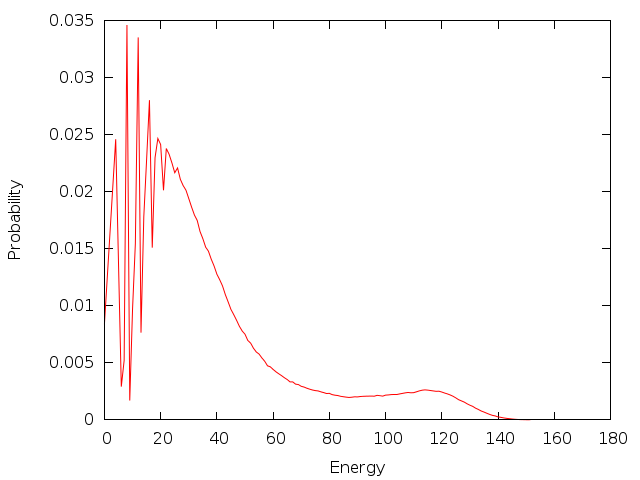
\includegraphics[height=6cm]{../results/metropolis/m10.png}}
\subfloat{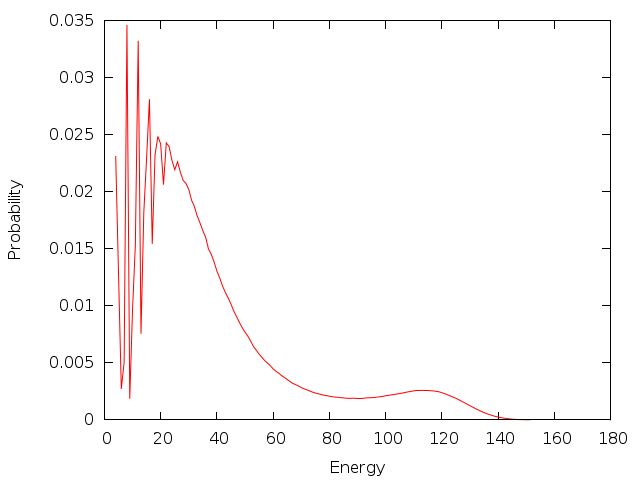
\includegraphics[height=6cm]{../results/wanglandau/b10.png}}
\label{fig:m10}
\end{figure}

\begin{figure}[h]
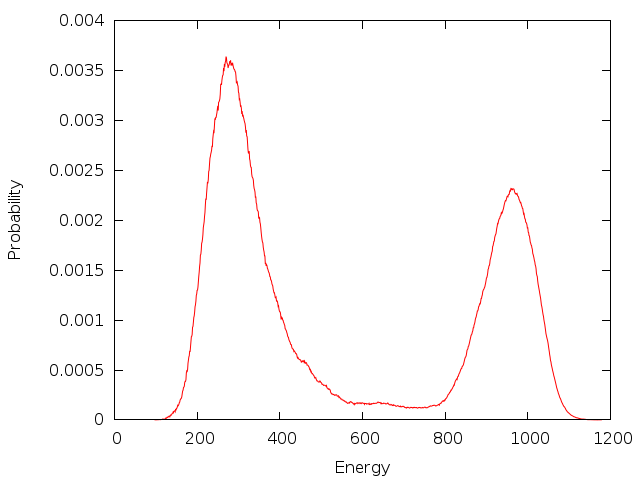
\includegraphics[height=8cm]{../results/metropolis/m30.png}
\caption{Boltzmann distribution for $l = 30$ (Metropolis)}
\label{fig:m30}
\end{figure}

\begin{figure}[h]
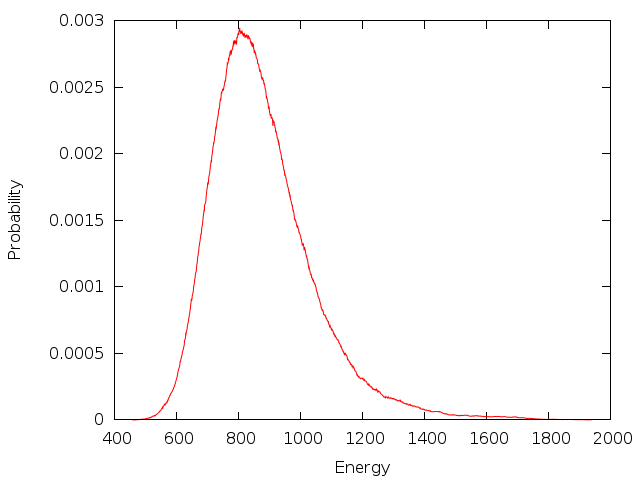
\includegraphics[height=8cm]{../results/metropolis/m50.png}
\caption{Boltzmann distribution for $l = 50$ (Metropolis)}
\label{fig:m50}
\end{figure}

\subsection{Wang-Landau}
For the Wang-Landau algorithm, we ran the algorithm with $f_1 = e$, and $f_i = \sqrt{f_{i-1}}$, with a final value of $f = e^{10^{-8}}$.
The number of ranges used in all cases was 15.

In figures \ref{fig:b10}, \ref{fig:b30}, and \ref{fig:b50}, we give the Boltzmann distributions obtained for lattice sizes $l = 10$, $l = 30$, and $l = 50$, respectively, obtained using the Wang-Landau algorithm and using $\beta = 1.424$.
These are provided for comparison with those obtained in section \ref{sec:metropolis}.

The actual data obtained directly from the Wang-Landau algorithm is the density of states.
We show the density of states obtained for $l = 10$ and $l = 30$ in figures \ref{fig:s10} and \ref{fig:s30}, respectively.

In figure \ref{fig:capacity}, we show the heat capacity for $l \in\{10,15,20,25,30\}$, using the calculation derived in section \ref{sec:calculations}.
As expected for a first-order phase transition, this has a sharp peak at the transition temperature.

\begin{figure}[h]
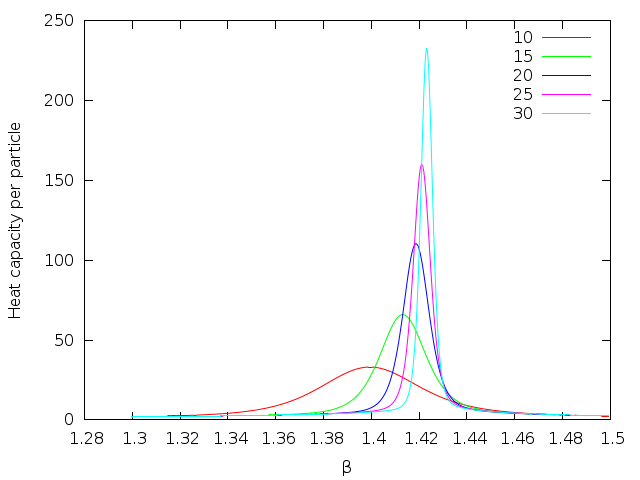
\includegraphics[height=8cm]{../results/wanglandau/capacity.png}
\caption{Heat capacity per particle $C = \frac{1}{l^2}\frac{\partial\langle E\rangle}{\partial T}$ for different $l$}
\label{fig:capacity}
\end{figure}

\begin{figure}[h]
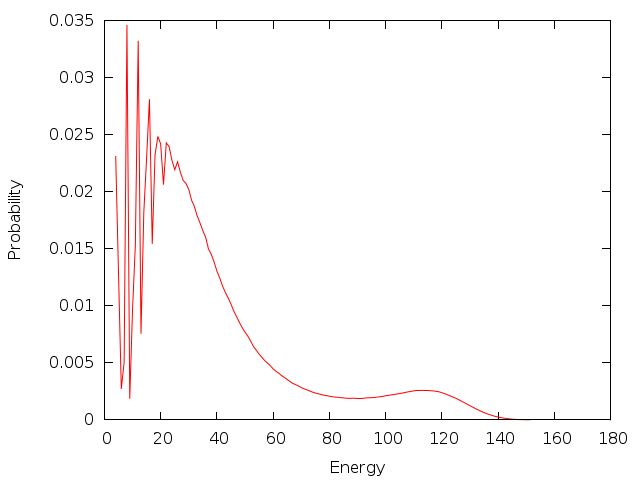
\includegraphics[height=8cm]{../results/wanglandau/b10.png}
\caption{Boltzmann distribution for $l = 10$ (Wang-Landau)}
\label{fig:b10}
\end{figure}

\begin{figure}[h]
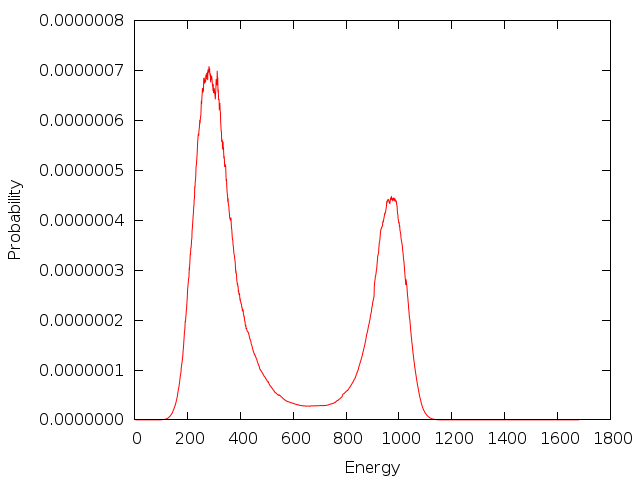
\includegraphics[height=8cm]{../results/wanglandau/b30.png}
\caption{Boltzmann distribution for $l = 30$ (Wang-Landau)}
\label{fig:b30}
\end{figure}

\begin{figure}[h]
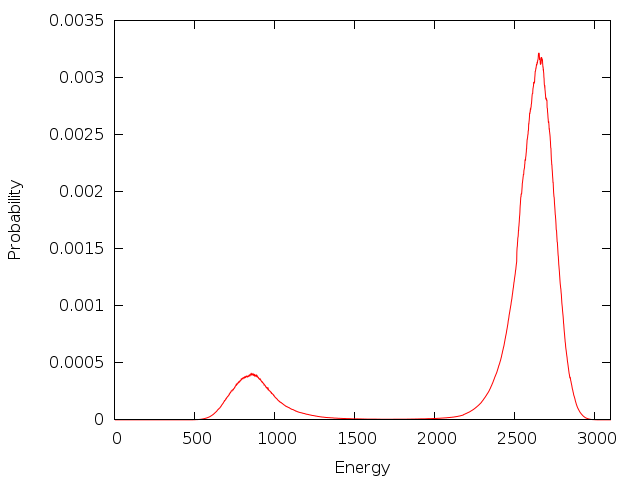
\includegraphics[height=8cm]{../results/wanglandau/b50.png}
\caption{Boltzmann distribution for $l = 50$ (Wang-Landau)}
\label{fig:b50}
\end{figure}

\begin{figure}[h]
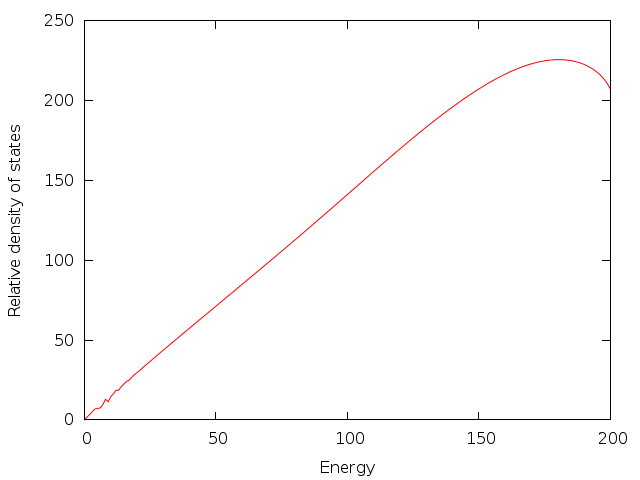
\includegraphics[height=8cm]{../results/wanglandau/s10.png}
\caption{Density of states for $l = 10$ (Wang-Landau)}
\label{fig:s10}
\end{figure}

\begin{figure}[h]
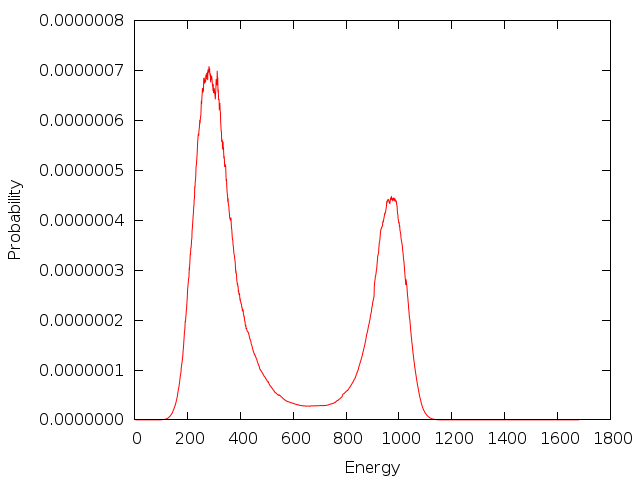
\includegraphics[height=8cm]{../results/wanglandau/s30.png}
\caption{Density of states for $l = 30$ (Wang-Landau)}
\label{fig:s30}
\end{figure}

\section{Discussion of results}
\subsection{Behavior for small lattices}
The behavior of the system for small lattice sizes was somewhat different to that for large lattice sizes at the same temperature.
We attempt to explain this here.

Firstly, the distribution for small lattice sizes did not appear to be evenly balanced between two phases at the supposed transition temperature $\beta = \log(1+\sqrt q)$, and in fact the ratio between the probabilities of the two phases varied as a function of lattice size.
This is just a consequence of the fact that this transition temperature is only asmyptotically valid \footnote{From figure \ref{fig:capacity}, the sequence of heat capacities per particle $C_l$ seems to have a monotonically increasing turning point, and to converge to a delta function for $l \rightarrow \infty$.}(moreover, at very small lattice sizes it is not clear that the phases are really distinct).

Secondly, the distribution for $l = 10$ was not a smooth distribution, instead having large fluctuations over small differences in $E$.
We explain this not as an effect of the lattice size, but rather just a consequence of the small energies involved, which we discuss more in the next section.

\subsection{Behavior for small energies}
For small energies the density of states does not have the same smooth behavior as at large energies.
This is because there are only a small number of possible ways (up to translation, rotation, reflection, and relabelling of spins) of obtaining each of these energies.

As an example, for lattices of size at least 2, the number of $E = 0$ states is $q$, and there are $0$ states for $E \in \{1,2,3,5\}$, but $l^2q^2$ states for $E = 4$.

\subsection{Convergence}
For the Metropolis algorithm, we obtained similar results to the Wang-Landau algorithm for $l \leq 30$.
In the $l = 50$ case, the distribution obtained at the transition temperature (given in figure \ref{fig:m50}) is clearly incorrect.
While the distribution looks reasonable for low energies, the high energy phase is missing.

This is a consequence of the fact that the Metropolis algorithm visits energies according to the Boltzmann distribution, and only moves between close energy levels.
The Potts model at the transition temperature contains a gap between the two phases in the Boltzmann distribution, where the system is unlikely to be.
Since the Metropolis algorithm must pass through this gap many times in order for the distribution to converge, and it is very unlikely to do so, the algorithm will take an impractical number of steps to converge.

\section{Conclusion}
\begin{thebibliography}{9}

\bibitem{WangLandau}
\newblock {\em {Efficient, Multiple-Range Random Walk Algorithm to Calculate the Density of States}},
\newblock F. Wang, D. P. Landau,
\newblock {\em {Physical Review Letters}}, 2001, Vol. 86, Part 10

\bibitem{Janke}
\newblock {\em {First-Order Phase Transitions}},
\newblock W. Janke,
\newblock {\em {Computer Simulations of Surfaces and Interfaces}}, NATO Science Series, II. Mathematics, Physics and Chemistry - Vol. 114, Proceedings of the NATO Advanced Study Institute, Albena, Bulgaria, 9 - 20 September 2002

\end{thebibliography}
\appendix
\section{Metropolis implementation}
\lstinputlisting[language=Python]{../metropolis.py}
\section{Wang-Landau implementation}
\lstinputlisting[language=Python]{../wanglandau1.py}
\end{document}
